\chapter{\label{results}Results and Discussion}
In the previous section, from \autoref{fig:fig}, we observed that the separation of the signal and the background events for different datasets were not clearly visible. This is a basic problem of classifications. To separate and make a proper visualization of the events as signal or background; there are several machine learning methods used traditionally, such as Boosted Decision Trees(BDTs), XGBoosts, and many other TMVA based machine learning methods. To separate signal and background, python based  modules such as Keras, which is based on the high-level wrapper for the machine learning frameworks Theano (\url{www.deeplearning.net/software/theano/}) and TensorFlow (\url{www.tensorflow.org}), they were mainly used to set up deep neural networks.\cite{29} \cite{30}
[\url{http:// tmva.sourceforge.net}]



\section{Uses of DNN }
The Deep Neural network(DNN) \footnote{All the code related to this work can be found here: \url{https://github.com/raj2022/M.Sc.-thesis/tree/main/Codes}} has been applied for training over the ntuple of tth, thq, ttgg and Tprime. The dataset was converted into the array using modules root2numpy(\url{https://scikit-hep.org/root_numpy/}), and further randomize it using rec2array. By using Pandas DataFrame we converted the array and further feed it into the model after splitting them as train and test data sets. The basic working model of the neural network is shown in the \autoref{fig:my_label_5.1}.
\begin{figure}[H]
    \centering
    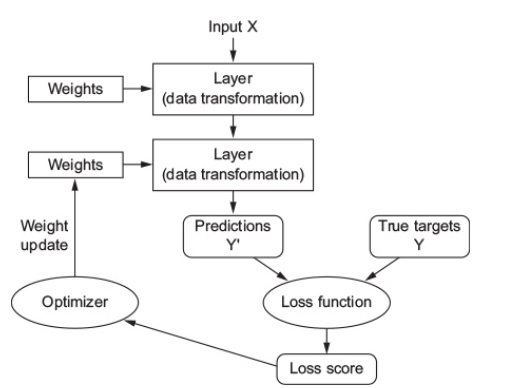
\includegraphics[scale=0.6]{Inputs/12__ml.png}
    \caption{Neural network scheme. Image source: [Chollet, 2017]}
    \label{fig:my_label_5.1}
\end{figure}

\section{DNN model}
Deep neural network (DNN) is used here for training the data and further testing the model. Keras module, Sequential used to make the DNN model. The basic architecture of our model are as follow, given in \autoref{tab:my_label_00}. Our model was made to train total 5,33,457 trainable parameters,and we also have total number of datasets around this number. The model was given total of 29 different input features( \autoref{tab:my_label_1}) in the first layer. To make neural layer more deep and to get a better training output, there were 4 extra hidden layers consisting of 200, 100, 100 and 100 nodes were added to the input layer. The output of successive layers goes as input to the next layer after passing through the  ReLU activation function(as shown in \autoref{fig:my_label_3}). For each layer, we have used dropout layer to save our model from collapsing.  For each 3 input model will drop a value, the model architecture is shown in the \autoref{fig:my_label_arch}.\\

For each input layers, we have provided weight or random state as 5, which will be getting updated after each training. The rationale behind choose these specific parameters such as the number of nodes, layers, epochs is to improve our training accuracy, and it was completely based on hit and trail method. \\

The output layer consist  only a single node for binary classification and again changed for multi classification, depending on the number of outputs we required as the outputs. In this semester project report, the output will only behave either as signal or as background. The  output layer also depend on whether the output required in binary or multiclass. For binary classification, the common activation function used is 'sigmoid', which we have already discussed in \autoref{subsection:Activationfunction} 
The model was compile with the binary cross entropy loss function \& categorical\_crossentropy loss function depending on the type of classifications. To avoid the model collapsing issues, we have used ADAM optimizer in the model and to prevent the training from over-fitting, the model is trained with accuracy matrices.\\

The model was fitted with the given dataset by splitting it into training and testing dataset in the ratio of 80:20, that is 80\% of the data used for training and 20\% of the data used for testing the model. The model has also provided with validation dataset, which is sample of dataset used to provide an unbiased evaluation of a model fit on training dataset while having model hyper-parameter(discussed in \autoref{tab:my_label_00}. Here the validation dataset are one-fourth of training data. This model was trained in the batch of 900, which means for every training, it would divide the dataset into 900 mini batches and run through all over the training data. The number of epochs of the model is 100, it employs the model has run through 100 times in total, after each run, model update or optimize its weight/ random\_state by itself  depending on the output of the error/loss and other hyper parameter. The model was further tested on the given testing dataset.  
   
   
 \begin{figure}[H]
     \centering
     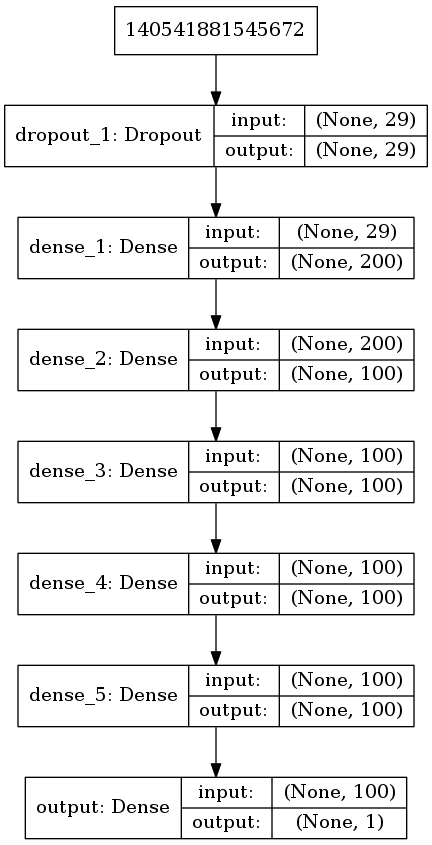
\includegraphics[scale=0.2]{TPrime_ttgg/clf_plot____.png}
     \caption{Basic architecture of our DNN Model }
     \label{fig:my_label_arch}
 \end{figure}
 %%%%%%%%%%%%%%%%%%Table Describing the model%%%%%%%%%%%%%%%%%%%%%%%%%%%%%%%%%%%%%%%%%%%%%%%%%%%%%%
 \begin{table}[H]
     \centering
     \begin{tabular}{|ccc|}\hline
       Options   &   & Description \\\hline
    Model      &    sequential  &   -   \\
    Number of Inputs      &    29  &    as given in \autoref{tab:my_label_1}  \\
    Number of layers (Input)     & 200     &  $Dense_1$    \\
        Hidden  &  200    &  $Dense_2$    \\
         Hidden &  100    &   $Dense_3$   \\
        Hidden  & 200     &  $Dense_4$    \\
        Hidden  & 200     & $Dense_5$     \\
        Output  & 1      &  $Dense_6$    \\
    Activation function(Hidden Layer)      &  ReLU    &   Same for both binary\\  
    & & classification and multiclassification   \\
      Activation layer(Output)    & sigmoid     &  For binary classification    \\
                                  &  Softmax  & For multi classification    \\
    Loss function   &   Binary cross entropy    & For binary classification \\
                    &    categorical\_crossentropy  & For multi classification \\
    Optimizer      &     ADAM     &     -\\
    Matrices     & Accuracy    &  \\
    BatchSize      & 900  & Batch size used for a single gradient  \\
                      &    &     step during training  \\
    NumEpochs      & 100 &   Number of training epochs \\
    Verbose &    1  &  Verbosity during training \\\hline
    
     \end{tabular}
     \caption{Configurations of the Keras model used for training and testing purposes}
     \label{tab:my_label_00}
 \end{table}
   
\section{Correlation between signal and background variable}
A correlation function represents a measurement between the strength of a linear relationship between two quantitative variables. There are two types of correlation, positive correlation and negative correlation. Positive correlation represents a relationship between two variables in which both variables move in the same direction. This means when one variable increases while the other also increases and vice versa While negative correlation is a relationship where one variable increases as the other decreases, and vice versa. A correlation of 1 or +1 shows a perfect positive correlation, which means both the variables move in the same direction. A correlation of -1 shows a perfect negative correlation, which means as one variable goes down, the other goes up \cite{27}. Here for the comparison of the variables (given in \autoref{tab:my_label_1}) from two different datasets were calculated using Pearson Correlation Coefficient Formula, which is,
\begin{equation}
    r = \frac{n(\sum xy)- \sum x \sum y}{\sqrt{[n \sum x^2 - (\sum x)^2][n \sum y^2 - (\sum y)^2]}}
\end{equation}
Where,\\
n = Quantity of Information \\
$\sum x$ = Total of the First Variable Value \\
$\sum y$ = Total of the Second Variable Value\\
$\sum xy$ = Sum of the Product of first \& Second Value\\
$\sum x^2$ = Sum of the Squares of the First Value\\
$\sum y^2$ = Sum of the Squares of the Second Value\\

The correlation plot for the given variables of Tprime and ttgg are plotted in the \autoref{fig:example_correlation}.
  \begin{figure}[H]
    \centering
    \subfloat[\centering Background(ttgg)]{{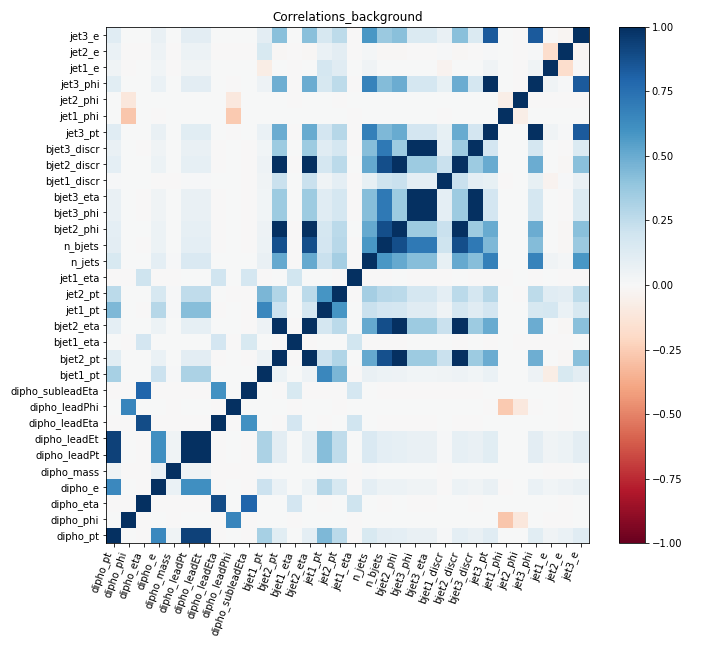
\includegraphics[width=10cm]{TPrime_ttgg/new_correlation_background.png} }}%
    \qquad
    \subfloat[\centering Signal(Tprime)]{{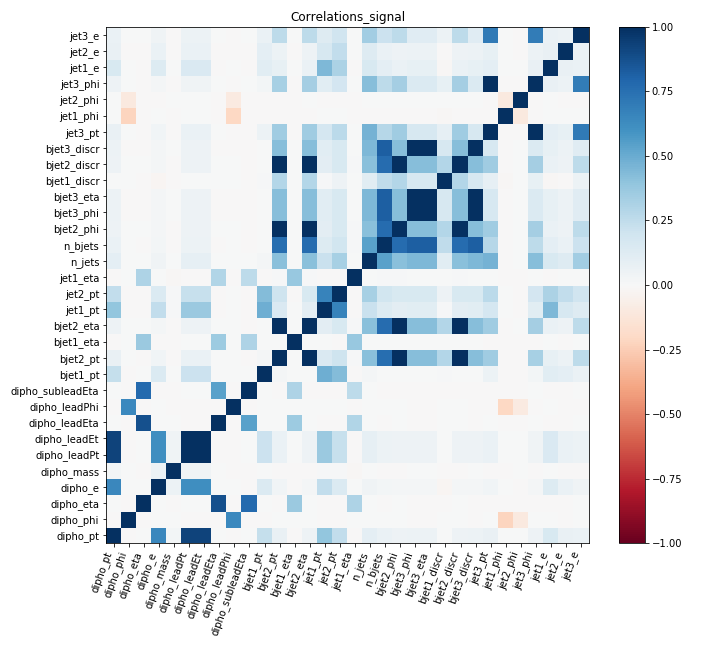
\includegraphics[width=10cm]{TPrime_ttgg/new_correlation_signal.png} }}%
    \caption{Correlation plot of two different datasets for different variables. Above, (a) Correlation plot for background(ttgg) and below, (b) Correlation plot for signal(Tprime)}
    \label{fig:example_correlation}
\end{figure}

   \begin{table}[h!]
    \centering
    \begin{tabular}{|c|c|}\hline
     Sl. No.    & Variables \\\hline
       1  & dipho\_pt \\
        2  & dipho\_phi \\
         3  & dipho\_eta \\
          4  & dipho\_mass \\
           5  & dipho\_leadPt \\
            6  & dipho\_leadEt \\
             7  & dipho\_leadEta \\
              8  & dipho\_leadPhi \\
               9  & dipho\_subleadEta \\
                10  & bjet1\_pt \\
                 11  & bjet2\_pt \\
                  12  & bjet1\_eta \\
                   13  & bjet2\_eta \\
                    14  & jet1\_pt \\
                     15  & jet2\_pt \\
                      16  & jet1\_eta \\
                       17  & n\_jets \i\
                        18  & n\_bjets \\
                         19  & bjet2\_phi \\
                          20  & bjet3\_phi \\
                        %   1  & bjet3_eta \\
                            21  & bjet1\_discr \\
                             22  & bjet2\_discr \\
                              23  & bjet3\_discr \\
                              24 & jet3\_pt \\
                                % & jet1\_phi \\
                                % & jet2\_phi \\
                              25  & jet3\_phi \\
                                26  & jet1\_e \\
                                  27  & jet2\_e \\
                                    28  & jet3\_e \\ 
                                    29 & dipho\_e \\\hline
           
    \end{tabular}
    \caption{Variables of $\Bar{t}th$, Tprime(T'), thq, and ttgg used in separation of signal and Background}
    \label{tab:my_label_1}
\end{table}
   
 \section{Binary Classifications}
 
Using the above discussed DNN model, when fitted with batch size of 900, provided random state is 5 and epochs is 100 on the training dataset of Tprime and ttgg. We will obtain the output of signal and background as shown in the figure \autoref{fig:my_label_DNN_output}. The training and testing done using the deep neural network can be verified using the model accuracy and loss. The model training and testing loss and accuracy comparison have been shown in the \autoref{fig:my_label_00}  and  \autoref{fig:my_label_accuracy_ttgg} \\
 
   
\begin{figure}[H]
    \centering
    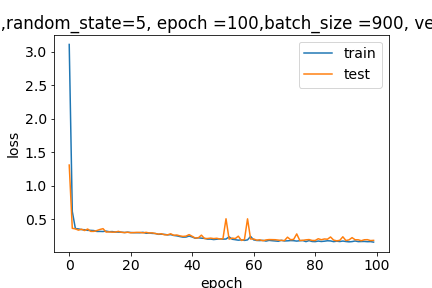
\includegraphics[scale=0.6]{TPrime_ttgg/loss_TPrime_ttgg.png}
    \caption{Training and testing loss when Tprime is used as signal and ttgg as the \\background}    \label{fig:my_label_00}
\end{figure}
%%%%%%%accuracy%%%%%%%%%%%%%
\begin{figure}[H]
    \centering
    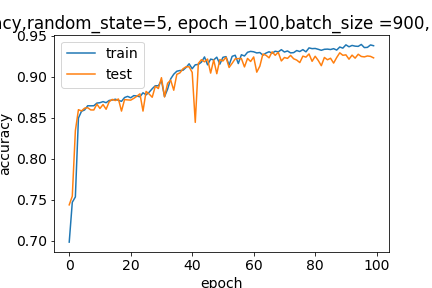
\includegraphics[scale=0.5]{TPrime_ttgg/accuracy_TPrime_ttgg.png}
    \caption{Training and testing model accuracy when Tprime is used as signal and ttgg as the background}
    \label{fig:my_label_accuracy_ttgg}
\end{figure}

%  The model output after training for signal and background separation are plotted in the fig. 5.7.  In this figure, our signal is plotted over 1 and rest background goes to zero.
 \begin{figure}[H]
     \centering
     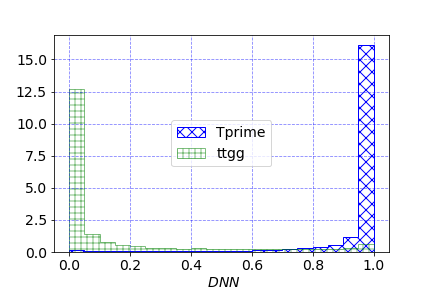
\includegraphics[scale=1]{TPrime_ttgg/output_TPrime_ttgg.png}
     \caption{Output of training using the DNN(Deep Neural Network). Here signal(Tprime) and background(ttgg) are clearly separated with background as 0 and signal corresponds to 1. }
     \label{fig:my_label_DNN_output}
 \end{figure}
 
 The performance analysis of the DNN model can be done with the help of the Receiving operator Characteristic(ROC) Curve plot for both the training and testing samples. The output ROC curve are plotted in the \autoref{fig:my_label_ROC_ttgg}
\begin{figure}[H]
    \centering
    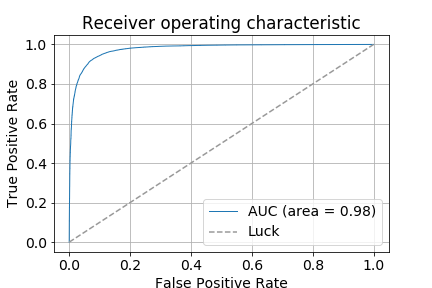
\includegraphics[scale=0.7]{ROC_curve_TPrime_ttgg.png}
    \caption{ROC curve for the training out of Tprime as signal and ttgg as the background}
    \label{fig:my_label_ROC_ttgg}
\end{figure}
%%%%%%%

For the comparison of the models, we can consider any other model of machine learning. Let's take infamous Boosted Decison Tree (BDT) model, it is used very frequently for data training at LHC. 
The BDT which can also distinguish between signal like and background like events. The output from this model of BDT classifier is plotted in \autoref{fig:my_label_BDT}. The area under the ROC Curve is 0.8863, while the training and testing output is around 82\% and 83 \% respectively. The input dataset for training and testing was T' and ttgg. The dataset was splitted over 33\% for the testing and 67\% for training. 


\begin{figure}[H]
    \centering
    \includegraphics[scale=0.7]{adaboost_classifier.png}
    \caption{Boosted Decision Tree(BDT), ROC curve  }
    \label{fig:my_label_BDT}
\end{figure}


 %%%%%%%%%%%%%%%%%
 
 Further, the model is used to train and test for the different combinations with the datasets. All the output scores of these training and testing are summarized in the \autoref{tab:my_label_0021}. The output plot for training with Tprime as signal and $\Bar{t}th$ \& ttgg as background plotted in \autoref{fig:my_label_000}. In this figure, we can see the Tprime (signal) corresponds to 1 (plotted in blue) while $\Bar{t}th$ \& ttgg as background corresponds to 0.
  
  \begin{figure}[H]
     \centering
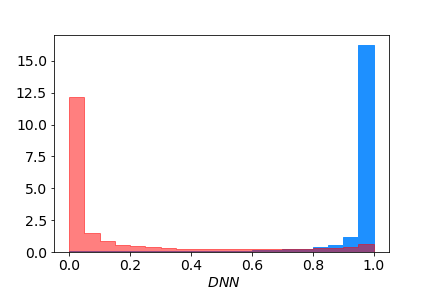
\includegraphics[scale=1]{TPrime_ttgg&tth&thq/output_TPrime_ttgg_&tth.png}
     \caption{Output of training from the DNN(Deep Neural Network). Here signal(Tprime) and background(ttgg  \& $\Bar{t}th$ ) are clearly separated with background as 0 and signal corresponds to 1. }
     \label{fig:my_label_000}
 \end{figure}
 
 
 With the combination of all the three datasets as the background (ttgg  \& $\Bar{t}th$ \& thq), and the Tprime as signal, we plotted the results. The ROC-curve for this setup is plotted in the \autoref{fig:my_label_89}, and the model accuracy \& loss are plotted in \autoref{fig:my_label_23} and \autoref{fig:my_label_009} respectively.
 
\begin{figure}[H]
    \centering
    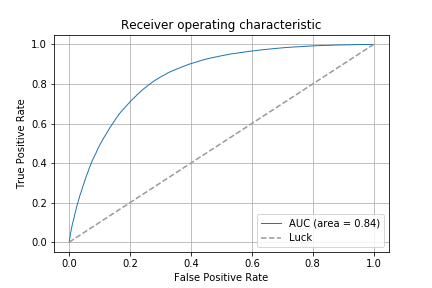
\includegraphics[scale=0.7]{TPrime_ttgg&tth&thq/ROC_curve_TPrime_ttgg_&tth&thq.png}
    \caption{ROC curve for the training output of Tprime as signal and ttgg, tth, and thq as the background}
    \label{fig:my_label_89}
\end{figure}

\begin{figure}[H]
    \centering
    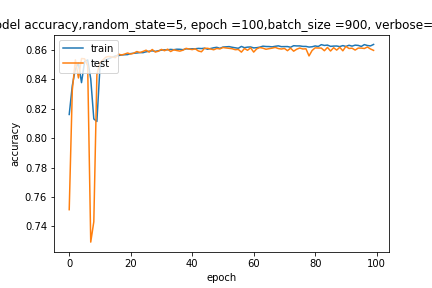
\includegraphics[scale=0.5]{TPrime_ttgg&tth&thq/model_accuracy_TPrime_ttgg_&tth&thq.png}
    \caption{Training and testing model accuracy when Tprime is used as signal and ttgg, tth, and thq were used as the background. To train different dataset over a single dataset are known as multi-class classification. }
    \label{fig:my_label_23}
\end{figure}

\begin{figure}[H]
    \centering
    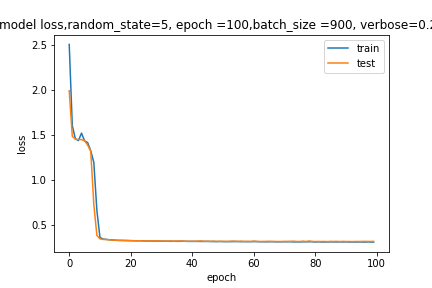
\includegraphics[scale=0.6]{TPrime_ttgg&tth&thq/loss_TPrime_ttgg_&tth&thq.png}
    \caption{Training and testing loss when Tprime is used as signal and ttgg, tth, and thq were used as the background. To train different dataset over a single dataset are known as multi-class classification. }
    \label{fig:my_label_009}
\end{figure}


%  \section{TPrime and ttgg}
%  \begin{figure}[H]
%     \centering
%     \subfloat[\centering label 1]{{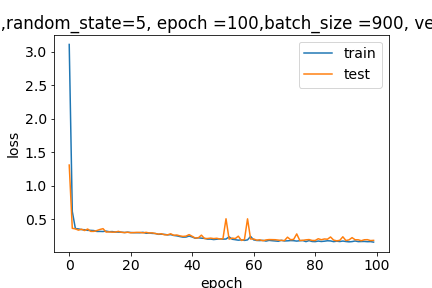
\includegraphics[width=5cm]{TPrime_ttgg/loss_TPrime_ttgg.png} }}%
%     \qquad
%     \subfloat[\centering label 2]{{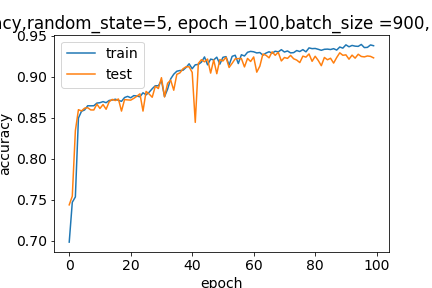
\includegraphics[width=5cm]{TPrime_ttgg/accuracy_TPrime_ttgg.png} }}%
%     \caption{2 Figures side by side}%
%     \label{fig:example}%
% \end{figure}

%  \begin{figure}[H]
%      \centering
%      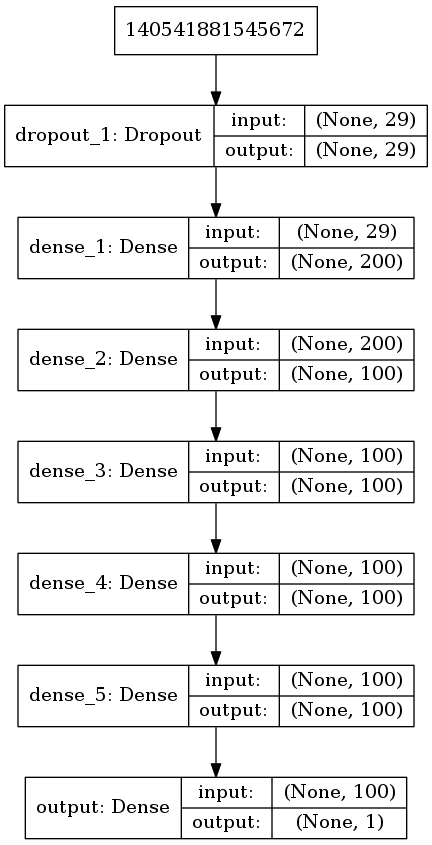
\includegraphics[scale=0.2]{TPrime_ttgg/clf_plot____.png}
%      \caption{Caption}
%      \label{fig:my_label}
%  \end{figure}
 
%  \begin{figure}[H]
%      \centering
%      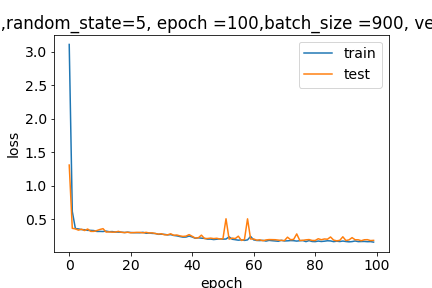
\includegraphics[scale=0.5]{TPrime_ttgg/loss_TPrime_ttgg.png}
%      \caption{Caption}
%      \label{fig:my_label}
%  \end{figure}

%   \begin{figure}[H]
%      \centering
%      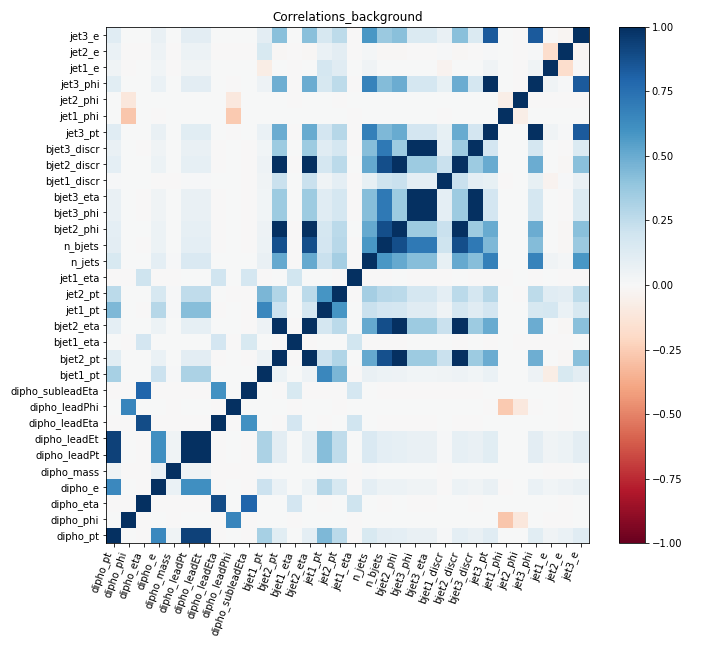
\includegraphics[scale=0.5]{TPrime_ttgg/new_correlation_background.png}
%      \caption{Caption}
%      \label{fig:my_label}
%  \end{figure}
 
 
%   \begin{figure}[H]
%      \centering
%      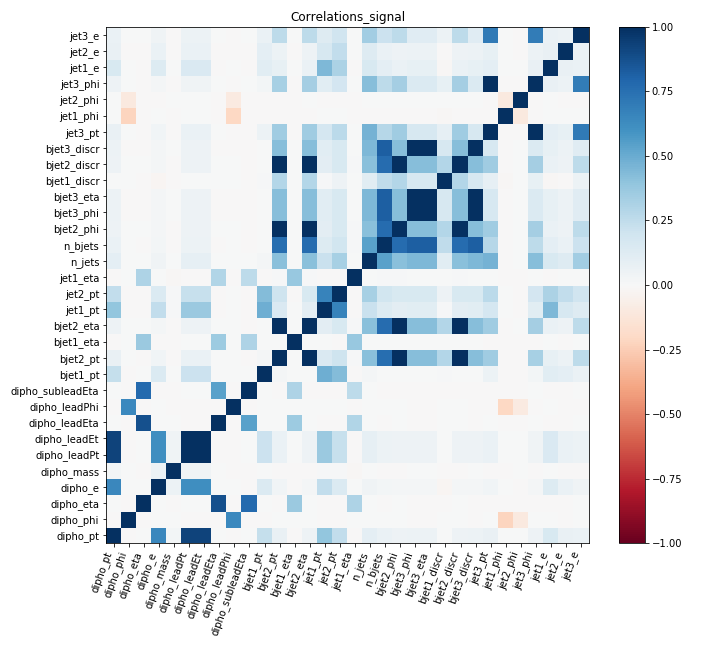
\includegraphics[scale=0.5]{TPrime_ttgg/new_correlation_signal.png}
%      \caption{Caption}
%      \label{fig:my_label}
%  \end{figure}
 


%  \begin{figure}[]
%      \centering
%      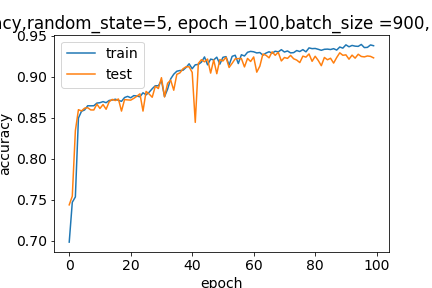
\includegraphics[scale=0.5]{TPrime_ttgg/accuracy_TPrime_ttgg.png}
%      \caption{Caption}
%      \label{fig:my_label}
%  \end{figure}
% \subsection{Correlation between signal and background variable}

\begin{table}[H]
    \centering
     \caption{Table with training and testing accuracy \%}
    \begin{tabular}{|c|c|c|c|}\hline
        Signal & Background & Training Accuracy(\%) & Testing Accuracy(\%) \\\hline
        TPrime & ttgg & 93.30 & 92.06  \\
        TPrime & ttgg\& tth & 89.84 & 89.07\\
        TPrime & ttgg\& tth\& thq & 86.36 & 86.10 \\ \hline
    \end{tabular}
    \label{tab:my_label_0021}
\end{table}

If we compare out DNN outputs for each process combination from the \autoref{tab:my_label_0021}, and also by comparing \autoref{fig:my_label_DNN_output} \& \autoref{fig:my_label_000}, we find that the training and testing accuracy are decreasing. To rectify these issues, we plan to implement multi-class classification, which we will be discussing this in the next section.
%%%%%%%%%%%%%%%%%%%%%%%%%%%%%%%%%%%%%%%%%%%%%%%%
%%%%%%%%%%%%%%%%%%%%%%%%%%%%%%%%%%
\section{Multi class Classification}
For the case of multi-class classification, we cannot use the same model of binary classifications(\autoref{tab:my_label_00}). We tried to create a different model, to avoid the frequent case of model collapsing, the model summary can be seen from \autoref{fig:multicalss} we try to use batch normalization and dropout layers after each dense layers. \dots 

\begin{wrapfigure}{l}{0.5\textwidth}
\centering
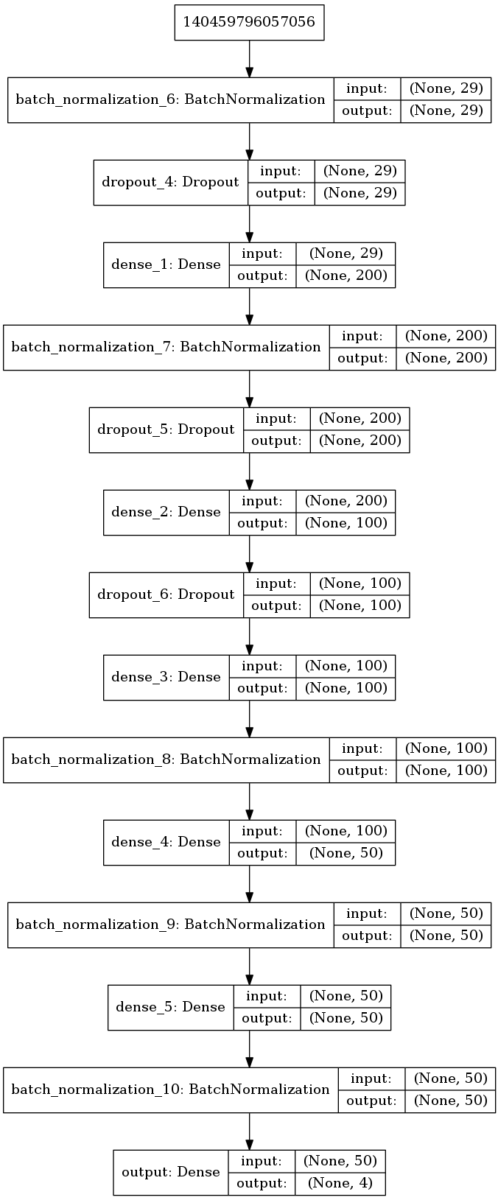
\includegraphics[width=.98\linewidth]{Inputs/clf_plot_multiclass___.png}
\caption{mode summary for the multi class classifications}
\label{fig:multicalss}
\end{wrapfigure}
% \lipsum[1]
The model obtains the same input variable, as the previous model for the binary classifications \autoref{fig:my_label_arch}. The  total number of input variables are 29 as given in \autoref{tab:my_label_1}. It is a general technique that can be used to normalize the inputs to a layer. We use first layer of batch normalization and divides the layers into mini batches. The output of this layer goes as input of the subsequent layer and we again use batch normalization and this continues till the output layer.The Output layer consists of 4 different outputs as we were dividing it into 4 different classes of Tprime($T^'$), $\Bar{t}th$, thq, and tt$\gamma \gamma$, respectively. \\
Deep neural networks(DNN) are sometimes very challenging to train, not least because the input from prior layers can change after weight update. Thus, by addition of batch normalization, it can be used to normalize the inputs given to a layer. The batch regularization accelerated the training rate and in some cases by halving the epochs or better. and further provides some regularization (two regularization, L1 and L2), and further reducing the generalization error.\\
The activation function used for inner layers were "ReLU", while the activation function for the output layer were "softmax". The corresponding loss function for multicalss training were "categorical\_crossentropy" with "ADAM" optimizer.

The training output of this model is plotted in the \autoref{fig:my_label_0099211} for accuracy and \autoref{fig:my_label-098365}, for model loss.


% \begin{figure}[htbp]
%   \raggedright
%     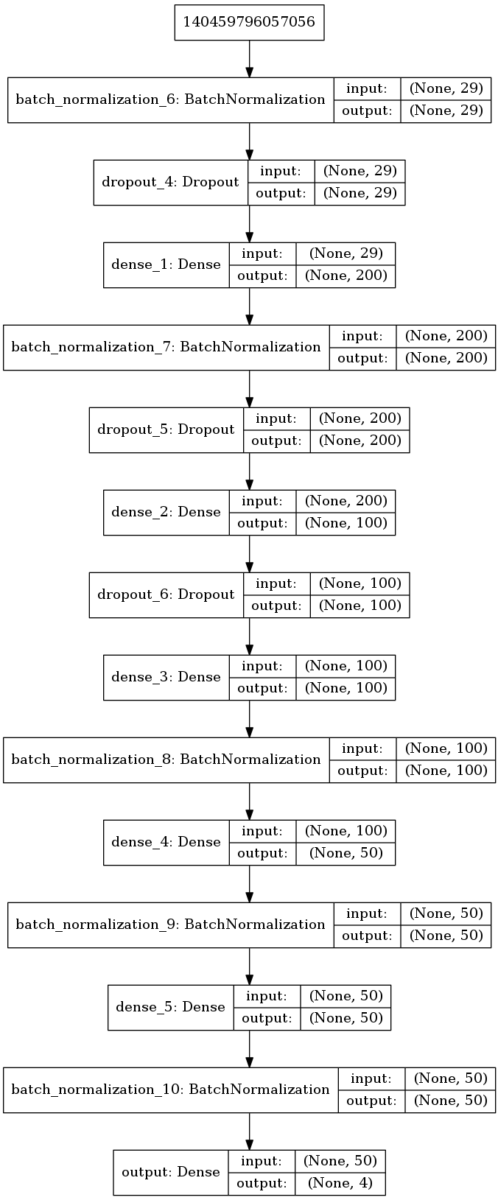
\includegraphics[scale=0.4]{Inputs/clf_plot_multiclass___.png}
%     \caption{Multiclass model summary}
%     \label{fig:my_label}
% \end{figure}


\begin{figure}[H]
    \centering
    \includegraphics[scale=0.7]{Model_accuracy_multiclass.png}
    \caption{Multiclass classification output for accuracy of training and testing}
    \label{fig:my_label_0099211}
\end{figure}


\begin{figure}[H]
    \centering
    \includegraphics[scale=0.7]{Model_loss_multiclass.png}
    \caption{Multiclass classification output for model loss of training and testing}
    \label{fig:my_label-098365}
\end{figure}
% \section{Mult-classification Outputs}
% Add the ROC curve 


% \setcounter{equation}{0}
% \setcounter{table}{0}
% \setcounter{figure}{0}
% %\baselineskip 24pt


    


% \subsection{Add following for better understanding}
% \begin{itemize}
%     \item Epoch change correpsonding to accuracy
% \end{itemize}


